\documentclass[11pt]{article}
\usepackage[margin=1in]{geometry}
\usepackage{graphicx}
\usepackage{amsmath}
\usepackage{booktabs}

\title{A Finite Intercept Correction Calculation}
\author{Anonymous}
\date{}

\begin{document}
\maketitle

\begin{abstract}
This teaching note connects residual averaging to least-squares intercept fitting for a fixed predictor. Five supplied observations satisfy $y_i=2x_i+3$, so the baseline $2x_i$ has constant residual $3$. Adding the mean residual reproduces every target. Exact mean absolute errors are $3,1.5,0$, and mean squared errors are $9,2.25,0$, at corrections $0,1.5,3$. A derivation, table, and two complementary figures illustrate fitting, error aggregation, and evaluation on the observations used for fitting.
\end{abstract}

\section{Introduction}

This worked example is intended for students beginning regression or machine learning who can manipulate sums and evaluate simple functions. Its educational objective is to connect four ideas: residuals as target-minus-prediction differences, intercept fitting with a fixed baseline, absolute versus squared error aggregation, and the role of observations in both fitting and evaluation.

The supplied construction makes every operation inspectable. Students can calculate the correction by hand, identify its least-squares objective, and trace which targets enter each stage. The central distinction is between making residuals average to zero and making every residual zero. The example achieves both because its baseline residuals are identical. Its contribution is an explicit instructional sequence linking these concepts.

\section{Related Work}

Eisenhauer discusses when regression through the origin is appropriate and how its evaluation depends on intercept conventions \cite{Eisenhauer2003RegressionThrough}. Here, the baseline slope remains fixed while an added intercept is fitted. Gneiting emphasizes matching an error measure to the forecasting task \cite{Gneiting2011MakingEvaluating}; squared error defines the fitting objective below, while absolute error provides a second summary. Efron examines apparent error when observations are used both to fit and to assess a prediction rule \cite{Efron1986HowBiased}. That dependency motivates the explicit evaluation path in our diagram. These references support the teaching concepts rather than serve as experimental competitors.

\section{Method}

\subsection{Finite Calculation and Error Definitions}

The supplied observations and fixed baseline predictions are
\[
\begin{aligned}
x&=(-2,-1,0,1,2),\\
y&=(-1,1,3,5,7),\\
\hat{y}^{(0)}&=(-4,-2,0,2,4).
\end{aligned}
\]
For $i=1,\ldots,5$, define the baseline residual
$r_i=y_i-2x_i$. Thus $r=(3,3,3,3,3)$.
Adding a scalar $b$ gives
\[
\hat{y}_i(b)=2x_i+b,
\qquad
e_i(b)=y_i-\hat{y}_i(b)=r_i-b.
\]
The summaries computed on these observations are
\[
\begin{aligned}
\operatorname{MAE}(b)&=\frac{1}{5}\sum_{i=1}^{5}|r_i-b|,\\
\operatorname{MSE}(b)&=\frac{1}{5}\sum_{i=1}^{5}(r_i-b)^2.
\end{aligned}
\]
Since every $r_i=3$, substitution gives
\[
\operatorname{MAE}(b)=|3-b|,
\qquad
\operatorname{MSE}(b)=(3-b)^2.
\]
These are algebraic consequences of the supplied targets and baseline.

\subsection{Mean Residual Correction and Computational Flow}

Fitting only the added intercept by least squares means minimizing
$\operatorname{MSE}(b)$ while keeping $2x_i$ fixed. Let
$\bar r=\frac{1}{5}\sum_i r_i$. Expanding the squares and using
$\sum_i(r_i-\bar r)=0$ yields
\[
\operatorname{MSE}(b)
=
\frac{1}{5}\sum_{i=1}^{5}(r_i-\bar r)^2
+
(b-\bar r)^2.
\]
The first term is independent of $b$, so the unique minimizer is
\[
b^\star=\bar r
=\frac{3+3+3+3+3}{5}=3.
\]
This is least-squares fitting of an intercept to the residuals of a fixed baseline, with no slope estimation. The identity separates residual centering from exact agreement: the corrected residuals sum to zero, whereas zero squared error requires every baseline residual to equal $\bar r$. The supplied residual vector satisfies that condition, giving
$\hat y(3)=y$.

Figure~\ref{fig:residual_workflow} provides a dependency view of the same calculation. Its solid arrows trace subtraction, averaging, and addition. Its dashed path lets students identify explicitly where the fitting observations re-enter evaluation.

\begin{figure}[!htbp]
    \centering
    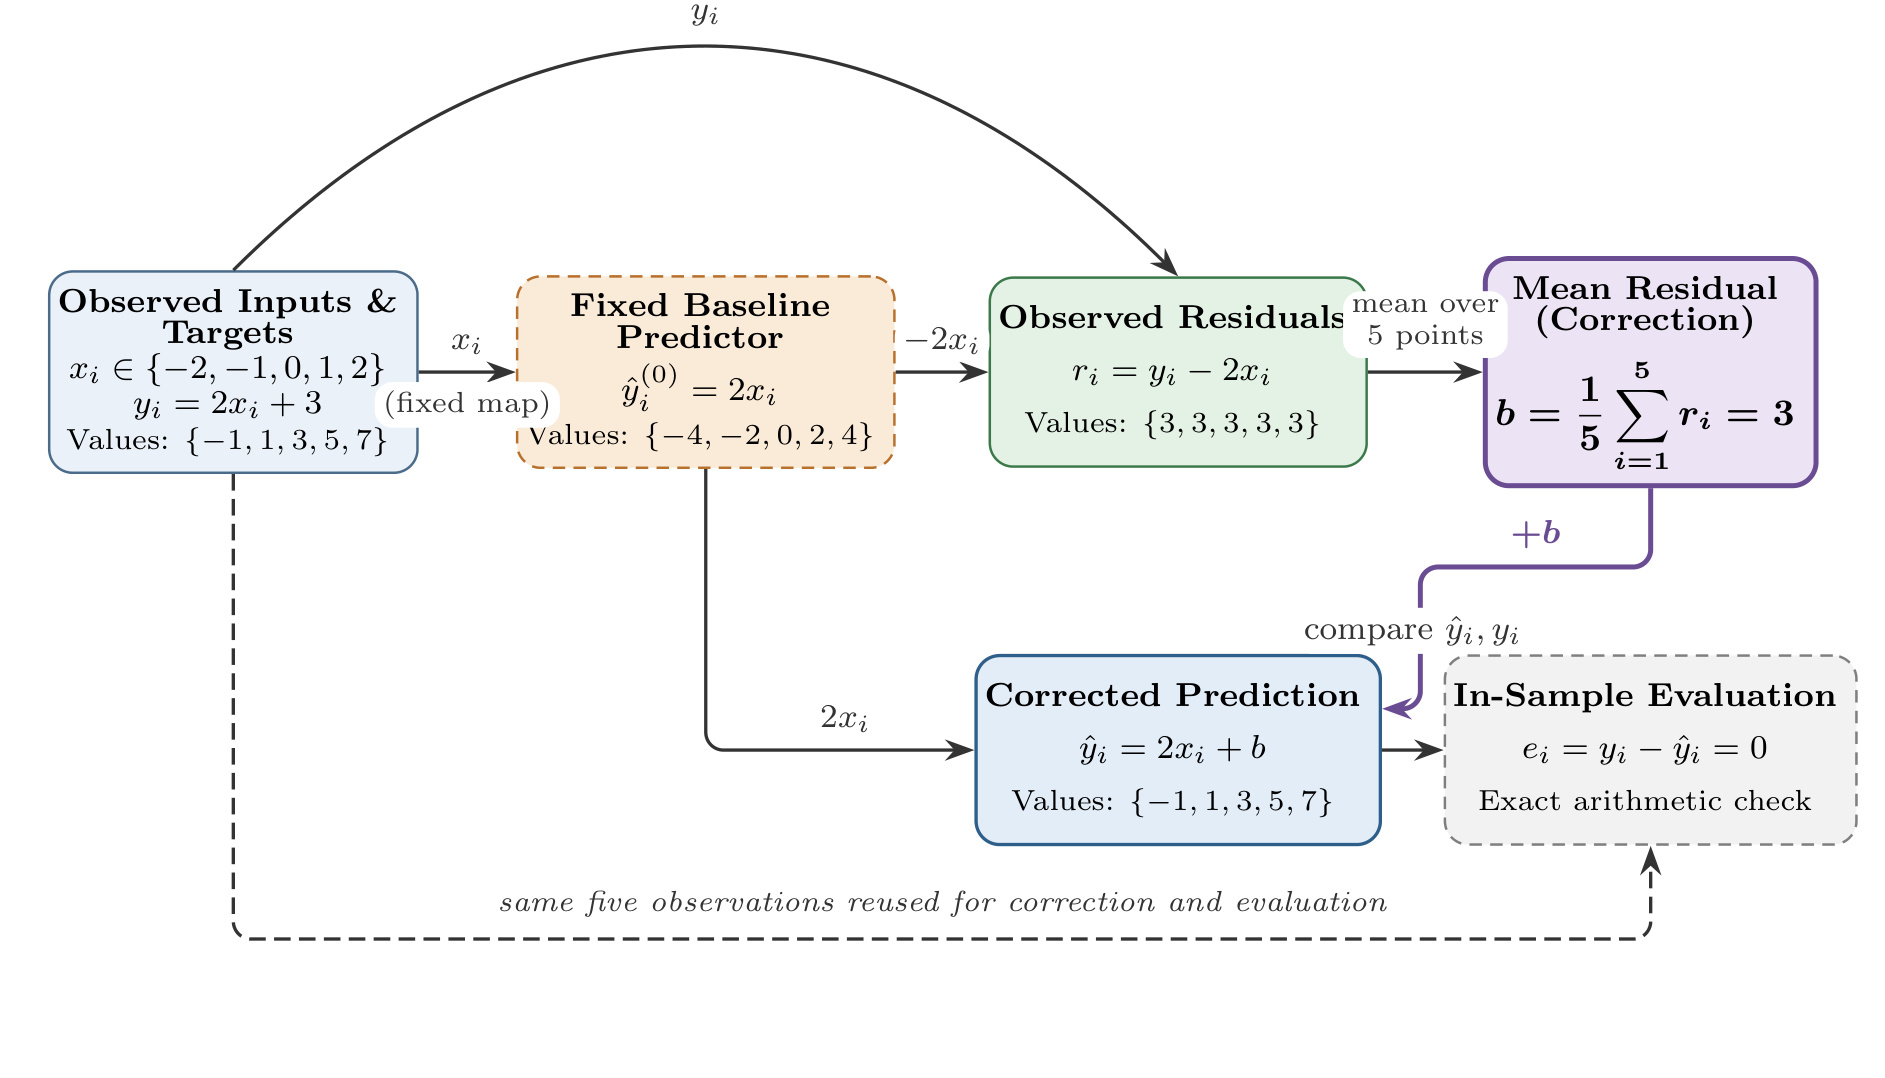
\includegraphics[width=\linewidth]{figures/fig_residual_workflow.jpg}
    \caption{Computational dependencies for the supplied five observations. Residual averaging fits the added intercept while preserving the baseline slope. The dashed path identifies the targets reused for evaluation.}
    \label{fig:residual_workflow}
\end{figure}

\section{Experiments}

\subsection{Observations and Evaluation Protocol}

The supplied base R calculation evaluates one deterministic construction. All five observations determine $b^\star$ and enter the error summaries. The three evaluated settings, $b=0,1.5,3$, represent the baseline, half the fitted correction, and the fitted correction. They are settings within the same calculation, rather than repeated trials.

The calculation directly averages residuals and evaluates predictions; it uses no iterative optimizer. Its outputs quantify arithmetic agreement with the targets that determine the correction. The least-squares derivation explains those outputs independently of the implementation.

\subsection{Exact Errors and Reproducible Figures}

Table~\ref{tab:recorded_errors} reproduces the numerical outputs of the supplied calculation. Every entry also follows exactly from the two error identities. At $b=1.5$, halving the common residual halves MAE and quarters MSE. At $b=3$, every residual vanishes. Thus the different numerical reductions illustrate absolute and squared aggregation of the same discrepancies.

\begin{table}[!htbp]
    \centering
    \caption{Exact error values computed on the five observations used to fit the correction.}
    \label{tab:recorded_errors}
    \begin{tabular}{rrr}
        \toprule
        Added $b$ & Mean absolute error & Mean squared error \\
        \midrule
        0   & 3   & 9    \\
        1.5 & 1.5 & 2.25 \\
        3   & 0   & 0    \\
        \bottomrule
    \end{tabular}
\end{table}

Figure~\ref{fig:intercept_error} supports comparison of the squared-error values, complementing the dependency diagram. The supplied R/ggplot2 source directly encodes the three tabulated pairs. It visualizes the calculation rather than providing an additional experiment. Only those three evaluated settings are plotted; the algebra supplies their explanation.

\begin{figure}[!htbp]
    \centering
    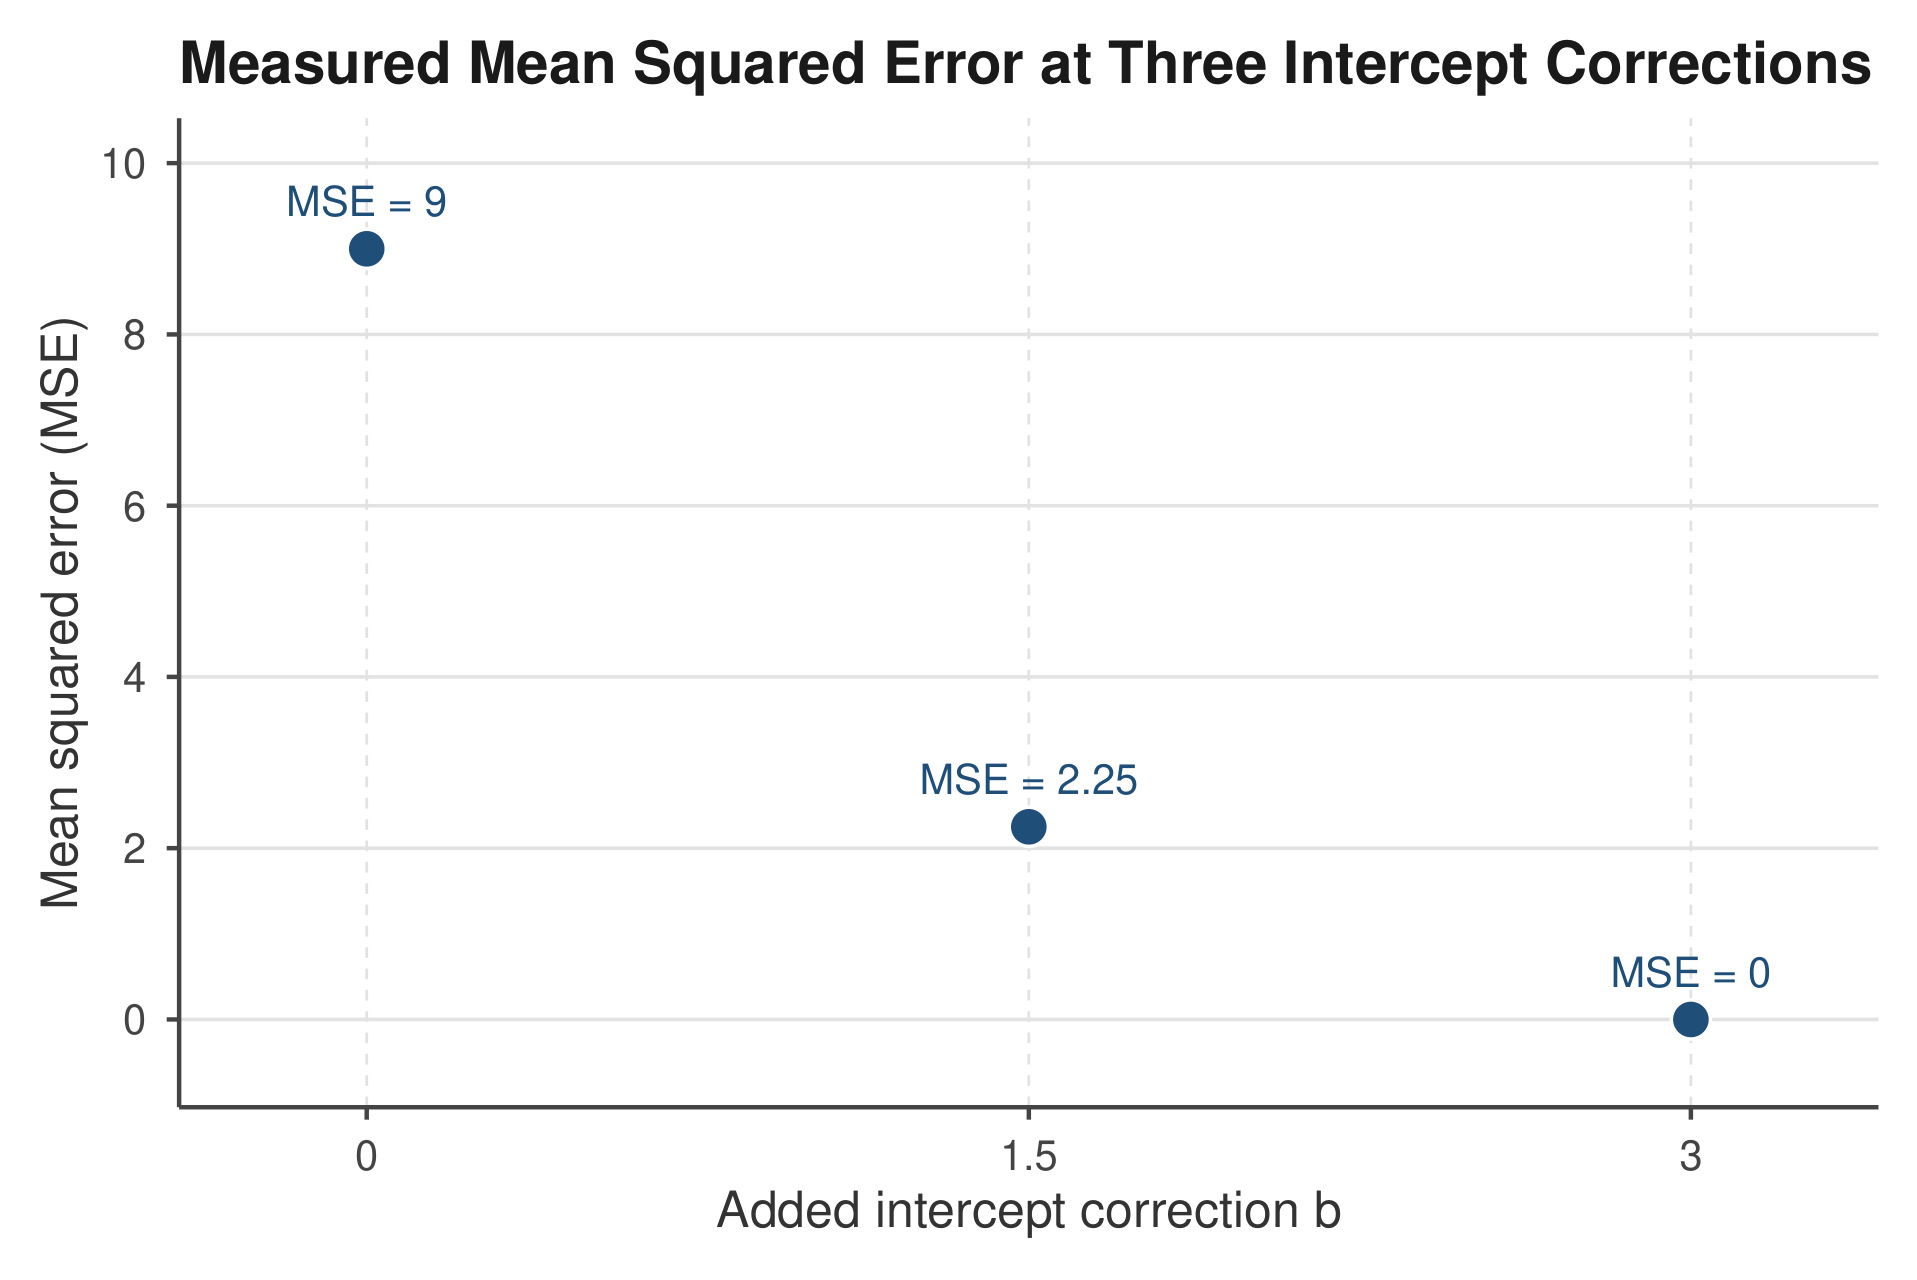
\includegraphics[width=\linewidth]{figures/fig_intercept_error.jpg}
    \caption{Exact evaluations $(b,\operatorname{MSE})=(0,9),(1.5,2.25),(3,0)$. The preserved title's ``Measured'' refers to these deterministic calculations. Each point summarizes the same five fitting observations.}
    \label{fig:intercept_error}
\end{figure}

\section{Conclusion}

The mean residual is the least-squares added intercept when the baseline predictions remain fixed. In this construction, identical baseline residuals make centering sufficient for exact agreement. The table distinguishes absolute from squared aggregation, while the figures connect numerical outputs to computational dependencies. Readers should leave able to derive the correction, explain why zero error occurs here, and identify precisely which observations the error summaries describe.


\begin{thebibliography}{9}

\bibitem{Eisenhauer2003RegressionThrough}
Joseph G. Eisenhauer.
\newblock Regression through the Origin.
\newblock \emph{Teaching Statistics}, 2003.

\bibitem{Gneiting2011MakingEvaluating}
Tilmann Gneiting.
\newblock Making and Evaluating Point Forecasts.
\newblock \emph{Journal of the American Statistical Association}, 2011.

\bibitem{Efron1986HowBiased}
Bradley Efron.
\newblock How Biased is the Apparent Error Rate of a Prediction Rule?
\newblock \emph{Journal of the American Statistical Association}, 1986.

\end{thebibliography}

% PAPER_ORCHESTRA_PROVENANCE_BEGIN
\clearpage
\section*{Figure source provenance}
The files below are the exact sources that produced the embedded figure previews. Paths are relative to this manuscript's source directory. The accompanying \texttt{figure\char95{}provenance.json} records all artifact checksums.\par
\medskip\noindent\textbf{Figure~\ref{fig:intercept_error} (\texttt{fig\char95{}intercept\char95{}error.jpg}).}\par
\noindent R/ggplot2 source: \texttt{figure\char95{}code/\allowbreak{}fig\char95{}intercept\char95{}error/\allowbreak{}source.R}.\par
\noindent Source SHA256: \texttt{2479e40e\allowbreak{}8d39e8e1\allowbreak{}6c29f883\allowbreak{}7e3b8df9\allowbreak{}909f9f65\allowbreak{}8bb35b95\allowbreak{}9fda0b12\allowbreak{}96debbe4}.\par
\noindent Rendering metadata: \texttt{figure\char95{}code/\allowbreak{}fig\char95{}intercept\char95{}error/\allowbreak{}render.json}.\par
\noindent Exact export wrapper: \texttt{figure\char95{}code/\allowbreak{}fig\char95{}intercept\char95{}error/\allowbreak{}worker.R}.\par
\noindent Wrapper SHA256: \texttt{1aedad4b\allowbreak{}1547d4b2\allowbreak{}d394cbb0\allowbreak{}239655d3\allowbreak{}667d453d\allowbreak{}d1fd0eca\allowbreak{}3e77c037\allowbreak{}e6d34892}.\par
\noindent Rendering metadata: \texttt{figure\char95{}code/\allowbreak{}fig\char95{}intercept\char95{}error/\allowbreak{}sessionInfo.txt}.\par
\medskip\noindent\textbf{Figure~\ref{fig:residual_workflow} (\texttt{fig\char95{}residual\char95{}workflow.jpg}).}\par
\noindent LaTeX/TikZ source: \texttt{figure\char95{}code/\allowbreak{}fig\char95{}residual\char95{}workflow/\allowbreak{}source.tex}.\par
\noindent Source SHA256: \texttt{84e305cc\allowbreak{}09efdeb2\allowbreak{}bc2162c3\allowbreak{}9fc60cb1\allowbreak{}d1a3c538\allowbreak{}4254d368\allowbreak{}dee04e8d\allowbreak{}b66664b4}.\par
\noindent Rendering metadata: \texttt{figure\char95{}code/\allowbreak{}fig\char95{}residual\char95{}workflow/\allowbreak{}render.json}.\par
% PAPER_ORCHESTRA_PROVENANCE_END
\end{document}